\subsection{Iteration for Nonlinear Systems(Optional)}

\frame{
Iterative techniques will now be discussed that extend the methods of Chapter 1 and Section 2.4 to the case of systems of nonlinear functions. 
Consider the functions 
\begin{equation*}
\begin{array}{l}
f_1(x,y) = x^2 - 2x - y + 0.5 \\
f_2(x,y) = x^2 + 4y^2 - 4
\end{array}
\end{equation*}
We seek a method of solution for the system of nonlinear equations 
\begin{equation*}
\begin{array}{l}
f_1(x,y) = 0 \\
f_2(x,y) = 0
\end{array}
\end{equation*}
}

\frame{
The equations $f_1(x, y) = 0$ and $f_2(x, y) = 0$ implicitly define curves in the $xy-$plane. 
Hence a solution of the system (2.51) is a point $(p, q)$ where the two curves cross (i.e., both $f_1(p, q) = 0$ and $f_2(P, q) = 0)$. \\
The curves for the system in (2.50) are well known: 
\begin{itemize}
\item $x^2 - 2x + 0.5 = 0$ is the graph of a parabola,
\item $x^2 + 4y^2 - 4 = 0$ is the graph of an ellipse.
\end{itemize}
\begin{figure}
\begin{center}
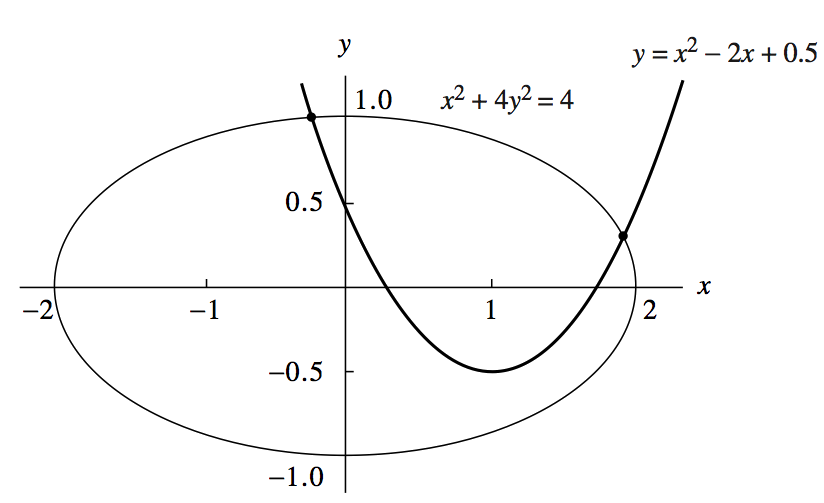
\includegraphics[width=70mm]{chap-2/fig_3-6.png}
\end{center}
\end{figure}
}

\frame{
\begin{itemize}
\item The first technique is fixed-point iteration.
\item A method must be devised for generating a sequence $\{ (p_k, q_k)\}$ that converges to the solution $(p, q)$. 
\item The first equation in (2.52) can be used to solve directly for $x$. 
\item However, a multiple of y can be added to each side of the second equation to get $x^2 + 4y^2 - 8y - 4 = -8y$. 
\item The choice of adding $-8y$ is crucial and will be explained later. 
\end{itemize}
We now have an equivalent system of equations: 
\begin{itemize}
\item $x  =  \frac{x^2 - y + 0.5}{2} $
\item $y  =  \frac{-x^2 - 4y^2 + 8y + 4}{8}$
\end{itemize}
}

\frame{
These two equations are used to write the recursive formulas. 
Start with an initial point $(p_0, q_0)$, and then compute the sequence $\{ (p_{k+1}, q_{k+1})\}$ using
\begin{itemize}
\item $p_{k+1}  =  \frac{p_k^2 - q_k + 0.5}{2} $
\item $q_{k+1}  =  \frac{-p_k^2 - 4q_k^2 + 8q_k + 4}{8}$
\end{itemize}
}

\frame{
If we use the starting value $(p_0, q_0) = (0, 1)$, then
\begin{itemize}
\item $p_1  =  \frac{0^2 - 1 + 0.5}{2} = -0.25$
\item $q_1  =  \frac{-0^2 - 4(1)^2 + 8(1) + 4}{8} = 1.0$
\end{itemize}
Iteration will generate the sequence  in case (i) of the following table. 
In this case the sequence converges to the solution that lies near the starting value $(0, 1)$. \begin{figure}
\begin{center}
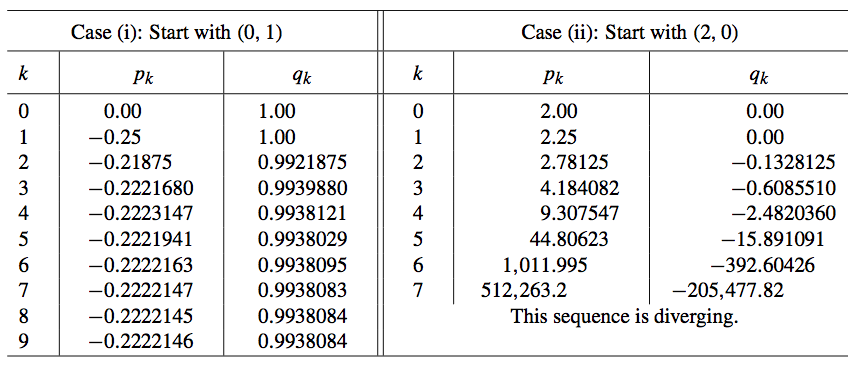
\includegraphics[width=60mm]{chap-2/tab_3-5.png}
\end{center}
\end{figure}
If we use the starting value $(p_0, q_0) = (2, 0)$, then
\begin{itemize}
\item $p_1  =  \frac{2^2 - 0 + 0.5}{2} = 2.25$
\item $q_1  =  \frac{-2^2 - 4(0)^2 + 8(0) + 4}{8} = 0.0$
\end{itemize}
Iteration will generate the sequence in case (ii) of  the above table. 
In this case the sequence diverges away from the solution.
}

\frame{
\begin{block}{}
\begin{itemize}
\item Iteration using formulas (2.54) cannot be used to find the second solution $(1.900677, 0.3112186)$. 
\item To find this point, a different pair of iteration formulas are needed. 
\item Start with equation (2.52) and add $-2x$ to the first equation and $-11y$ to the second equation and get 
\begin{equation*}
\begin{array}{l}
x^2 - 4x - y + 0.5 = -2x \\  
x^2 + 4y^2 - 11y - 4 = -11y. 
\end{array}
\end{equation*}
\end{itemize}
\end{block}
}

\frame{
These equations can then be used to obtain the iteration formulas
\begin{itemize}
\item $p_{k+1}  = g_1(p_k, q_k) =  \frac{-p_k^2 + 4 p_k + q_k - 0.5}{2} $
\item $q_{k+1}  = g_2(p_k, q_k) =  \frac{-p_k^2 - 4q_k^2 + 11q_k + 4}{11}$
\end{itemize}
\begin{figure}
\begin{center}
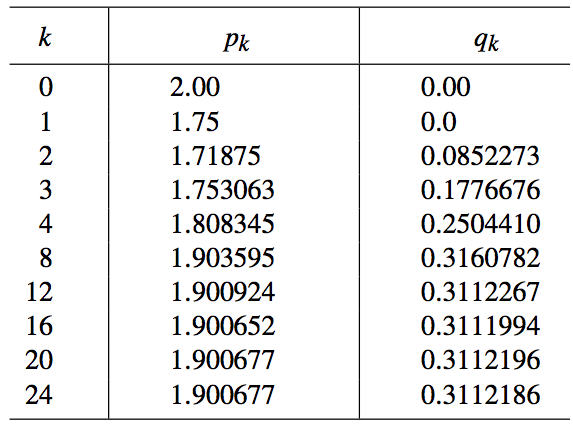
\includegraphics[width=80mm]{chap-2/tab_3-6.png}
\end{center}
\end{figure}
}

\frame{
\frametitle{Theory}
\begin{itemize}
\item We want to determine why equations (2.55) were suitable for finding the solution near (1.9,0.3) and equations (2.54) were not. 
\item In Section 1.1 the size of the derivative at the fixed point was the necessary idea. 
\item When functions of several variables are used, the partial derivatives must be used. 
\item The generalization of "the derivative" for systems of functions of several variables is the Jacobian matrix. 
\item We will consider only a few introductory ideas regarding this topic. 
\item More details can be found in any textbook on advanced calculus. 
\end{itemize}
}

\frame{
\begin{block}{Definition 2.6.}
 Assume that $f_1(x, y)$ and $f_2(x, y)$ are functions of the independent variables $x$ and $y$; then their {\Large Jacobian matrix}  $J(x, y)$ is
\begin{equation*}
\left[
\begin{array}{c c}
\frac{\partial f_1}{\partial x} & \frac{\partial f_1}{\partial y}\\
\frac{\partial f_2}{\partial x} & \frac{\partial f_2}{\partial y}
\end{array}
\right]
\end{equation*}
Similarly, if $f_1(x, y, z),$ $f_2(x, y, z)$, and $f_3(x, y, z)$ are functions of the independent variables $x$, $y$, and $z$, then their $3 \times 3$ Jacobian matrix $J(x, y, z)$ is defined  as follows:
\begin{equation*}
\left[
\begin{array}{c c c}
\frac{\partial f_1}{\partial x} & \frac{\partial f_1}{\partial y} & \frac{\partial f_1}{\partial z} \\
\frac{\partial f_2}{\partial x} & \frac{\partial f_2}{\partial y} & \frac{\partial f_2}{\partial z} \\
\frac{\partial f_3}{\partial x} & \frac{\partial f_3}{\partial y} & \frac{\partial f_3}{\partial z}
\end{array}
\right]
\end{equation*}
\end{block}
}

\frame{
\frametitle{Example 2.13}
Find the Jacobian matrix $J(x, y, z)$ of order $3 \times 3$ at the point $(1, 3, 2)$ for the three functions
\begin{equation*}
\begin{array}{r c l}
f_1 (x, y, z) & = & x^3 - y^2 + y -z^4 + z^2 \\
f_2 (x, y, z) & = & xy + yz + xz\\
f_3 (x, y, z) & = & y \slash xz
\end{array}
\end{equation*}

The Jacobian matrix is
\begin{equation*}
J(x, y, z) = 
\left[
\begin{array}{c c c}
\frac{\partial f_1}{\partial x} & \frac{\partial f_1}{\partial y} & \frac{\partial f_1}{\partial z} \\
\frac{\partial f_2}{\partial x} & \frac{\partial f_2}{\partial y} & \frac{\partial f_2}{\partial z} \\
\frac{\partial f_3}{\partial x} & \frac{\partial f_3}{\partial y} & \frac{\partial f_3}{\partial z} 
\end{array}
\right]
= 
\left[
\begin{array}{c c c}
3 x^2               & -2y+1         & -4z^3+2z \\
y+z                  & x+z             & y+x \\
\frac{-y}{x^2z} & \frac{1}{xz}  & \frac{-y}{xz^2} 
\end{array}
\right]
\end{equation*}
Thus the Jacobian evaluated at the point $(1, 3, 2)$ is the $3 \times 3$ matrix
\begin{equation*}
J(1,3,2) =
\left[
\begin{array}{c c c}
3               & -5             & -28 \\
5               &   3             & 4 \\
-\frac{3}{2} & \frac{1}{2}  & -\frac{3}{4} 
\end{array}
\right]
\end{equation*}
}


\frame{
\frametitle{Generalized Differential}
For a function of several variables, the differential is used to show how changes of the independent variables affect the change in the dependent variables. \\
Suppose that we have 
\begin{equation*}
\begin{array}{l}
u = f_1 (x, y, z), \\
v = f_2 (x, y, z), \\
w = f_3 (x, y, z).
\end{array}
\end{equation*}
}

\frame{
\begin{itemize}
\item Suppose that the values of the functions in (2.58) are known at the point $(x_0, y_0, z_0)$ and we wish to predict their value at a nearby point $(x, y, z)$. 
\item Let $du$, $dv$, and $dw$ denote differential changes in the dependent variables and $dx$, $dy$, and $dz$ denote differential changes in the independent variables. 
\item These changes obey the relationships 
\end{itemize}
\begin{equation*}
\begin{array}{l c l c l c l}
d u & = & \frac{\partial f_1}{\partial x} (x_0,y_0,z_0) dx & + & \frac{\partial f_1}{\partial y} (x_0,y_0,z_0) dy & + & \frac{\partial f_1}{\partial z}  (x_0,y_0,z_0) d_z\\
d v & = & \frac{\partial f_2}{\partial x} (x_0,y_0,z_0) dx & + & \frac{\partial f_2}{\partial y} (x_0,y_0,z_0) dy & + & \frac{\partial f_2}{\partial z} (x_0,y_0,z_0) d_z\\
d h & = & \frac{\partial f_3}{\partial x} (x_0,y_0,z_0) dx & + & \frac{\partial f_3}{\partial y} (x_0,y_0,z_0) dy & + & \frac{\partial f_3}{\partial z} (x_0,y_0,z_0) d_z
\end{array}
\end{equation*}
If vector notation is used, the above equations can be compactly written by using the Jacobian matrix. 
The function changes are $dF$ and the changes in the variables are denoted $dX$.
\begin{equation*}
d F = 
\left[
\begin{array}{c}
du \\
dv \\
dw 
\end{array}
\right]
= J (x_0,y_0,z_0)
\left[
\begin{array}{c}
dx \\
dy \\
dz
\end{array}
\right]
= J (x_0,y_0,z_0) d X
\end{equation*}
}


\frame{
\frametitle{Example 2.14}
Use the Jacobian matrix to find the differential changes $(du, dv, dw)$ when the independent variables change from $(1, 3, 2)$ to $(1.02, 2.97, 2.01)$ for the system of functions
\begin{equation*}
\begin{array}{r c l}
f_1 (x, y, z) & = & x^3 - y^2 + y -z^4 + z^2 \\
f_2 (x, y, z) & = & xy + yz + xz\\
f_3 (x, y, z) & = & y \slash xz
\end{array}
\end{equation*}
\begin{center}
$\Downarrow$
\end{center}
\begin{equation*}
\left[
\begin{array}{c}
du \\
dv \\
dw 
\end{array}
\right]
= 
\left[
\begin{array}{c c c}
3       & -5 & -28 \\
5       & 3 & 4\\
-\frac{3}{2} & \frac{1}{2} & -\frac{3}{4}
\end{array}
\right]
\left[
\begin{array}{c}
0.02 \\
-0.03 \\
0.01 
\end{array}
\right]
= 
\left[
\begin{array}{c}
-0.07 \\
  0.05 \\
-0.0525 
\end{array}
\right]
\end{equation*}
}

\frame{
\begin{center}
$\Downarrow$
\end{center}
Notice that the function values at $(1.02, 2.97, 2.01)$ are close to the linear approximations obtained by adding the differentials 
\begin{equation*}
\begin{array}{l c l}
du  & = & -0.07, \\ 
dv  & = & 0.05, \\
dw & = & -0.0525
\end{array}
\end{equation*}
 to the corresponding function values $f_1(1, 3, 2) = -17$, $f_2(1, 3, 2) = 11$, and $f_3(1, 3, 2) = 1.5$
\begin{center}
$\Downarrow$
\end{center}
\begin{equation*}
\begin{array}{l c r c r c l}
f_1(1.02, 2.97, 2.01) & = & -17.072 & \approx & -17.07 & = & f_1(1, 3, 2) + du \\
f_2(1.02, 2.97, 2.01) & = & 11.0493 & \approx & 11.05 & = & f_2(1, 3, 2) + dv \\
f_3(1.02, 2.97, 2.01) & = & 1.44864 & \approx & 1.4475 & = & f_3(1, 3, 2) + dw
\end{array}
\end{equation*}
}



\frame{
\frametitle{Convergence near Fixed Points}
\begin{itemize}
\item The extensions of the definitions and theorems in Section 1.1 to the case of two and three dimensions are now given. 
\item The notation for N-dimensional functions has not been used. 
\item The reader can easily find these extensions in many books on numerical analysis. 
\end{itemize}
}

\frame{
\begin{block}{Definition 2.7.}
 A {\Large fixed point} for the system of two equations
\begin{equation*}
\begin{array}{c c l}
x & = & g_1(x,y) \\ 
y & = & g_2(x,y)
\end{array}
\end{equation*}
is a point $(p, q)$ such that $p = g_1(p, q)$ and $q = g_2(p, q)$. 
Similarly, in three dimensions a fixed point for the system
\begin{equation*}
\begin{array}{c c l}
x & = & g_1(x,y,z) \\ 
y & = & g_2(x,y,z) \\
y & = & g_3(x,y,z)
\end{array}
\end{equation*}
is a point $(p, q, r )$ such that $p = g_1(p, q, r )$, $q = g_2(p, q, r )$, and $r = g_3(p, q, r )$.
\end{block}
}

\frame{
\begin{block}{Definition 2.8.}
For the functions defined in definition 2.7, {\Large fixed-point iteration} is
\begin{equation*}
\begin{array}{c c l}
p_{k+1} & = & g_1(p_k,q_k) \\ 
q_{k+1} & = & g_2(p_k,q_k)
\end{array}
\end{equation*}
for $k = 0, 1, \ldots $. \\
\vspace{3mm}
or
\begin{equation*}
\begin{array}{c c l}
p_{k+1} & = & g_1(p_k,q_k,r_k) \\ 
q_{k+1} & = & g_2(p_k,q_k,r_k) \\
r_{k+1}  & = & g_3(p_k,q_k,r_k)
\end{array}
\end{equation*}
for $k = 0, 1, \ldots $. \\
\end{block}
}

\frame{
\begin{block}{Theorem 2.9 (Fixed-Point Iteration).}
Assume that the functions in definition 2.7 and their first partial derivatives are continuous on a region that contains the fixed point $(p, q)$ or $(p, q, r )$, respectively. 
If the starting point is chosen sufficiently close to the fixed point, then one of the following cases applies. \\
Case (i): Two dimensions.
If $(p_0, q_0)$ is sufficiently close to $(p, q)$ and if
\begin{equation*}
\left| \frac{\partial g_1}{\partial x}(p,q)  \right|  +  \left| \frac{\partial g_1}{\partial y}(p,q)  \right|  <  1 
\end{equation*}
\begin{equation*}
\left| \frac{\partial g_2}{\partial x}(p,q)  \right|  +  \left| \frac{\partial g_2}{\partial y}(p,q)  \right|  <  1 
\end{equation*}
then the iteration in definition 2.8 converges to the fixed point $(p, q)$.
\end{block}
}

\frame{
\begin{block}{}
Case (ii): Three dimensions.
If $(p_0, q_0, r_0)$ is sufficiently close to $(p, q, r )$ and if
\begin{equation*}
\left| \frac{\partial g_1}{\partial x}(p,q,r) \right|  +  \left| \frac{\partial g_1}{\partial y}(p,q,r) \right|   +  \left| \frac{\partial g_1}{\partial r}(p,q,r) \right|   <  1 
\end{equation*}
\begin{equation*}
\left| \frac{\partial g_2}{\partial x}(p,q,r) \right|  +  \left| \frac{\partial g_2}{\partial y}(p,q,r) \right|   +  \left| \frac{\partial g_2}{\partial r}(p,q,r) \right|   <  1 
\end{equation*}
\begin{equation*}
\left| \frac{\partial g_3}{\partial x}(p,q,r) \right|  +  \left| \frac{\partial g_3}{\partial y}(p,q,r) \right|   +  \left| \frac{\partial g_3}{\partial r}(p,q,r) \right|   <  1 
\end{equation*}
then the iteration indefinition 2.8 converges to the fixed point $(p, q, r )$.
\end{block}
If conditions are not met, the iteration might diverge. 
This will usually be the case if the sum of the magnitudes of the partial derivatives is much larger than 1.
}

\frame{
\frametitle{Seidel Iteration}
An improvement, analogous to the Gauss-Seidel method for linear systems, of fixedpoint iteration can be made.
Suppose that $p_{k+1}$ is used in the calculation of $q_{k+1}$\footnote{in three dimensions both $p_{k+1}$ and $q_{k+1}$ are used to compute $r_{k+1}$}.
When these modifications are incorporated in formulas in definition 2.8, the method is called {\Large Seidel iteration}:
\begin{equation*}
\begin{array}{c c l}
p_{k+1} & = & g_1(p_k,q_k) \\ 
q_{k+1} & = & g_2(p_{k+1},q_k)
\end{array}
\end{equation*}
for $k = 0, 1, \ldots $. \\
\vspace{3mm}
or
\begin{equation*}
\begin{array}{c c l}
p_{k+1} & = & g_1(p_k,q_k,r_k) \\ 
q_{k+1} & = & g_2(p_{k+1},q_k,r_k) \\
r_{k+1}  & = & g_3(p_{k+1},q_{k+1},r_k)
\end{array}
\end{equation*}
for $k = 0, 1, \ldots $. 
}

\frame{
\frametitle{Newton's Method for Nonlinear Systems}
\begin{itemize}
\item We now outline the derivation of Newton's method in two dimensions. 
\item Newton's method can easily be extended to higher dimensions. 
\item Consider the system
\end{itemize} 
\begin{equation*}
\begin{array}{c c l}
u & = & f_1(x,y) \\ 
v & = & f_2(x,y)
\end{array}
\end{equation*}
which can be considered a transformation from the $xy-$plane to the $uv-$plane. 
}

\frame{
\begin{itemize}
\item We are interested in the behavior of this transformation near the point $(x_0, y_0)$ whose image is the point $(u_0, v_0)$. 
\item If the two functions have continuous partial derivatives, then the differential can be used to write a system of linear approximations that is valid near the point $(x_0, y_0)$: 
\end{itemize}
\begin{equation*}
u -u_0 \approx \frac{\partial}{\partial x}  f_1(x_0,y_0) (x - x_0)  + \frac{\partial}{\partial y}  f_1(x_0,y_0) (y - y_0) 
\end{equation*}
\begin{equation*}
v -v_0 \approx \frac{\partial}{\partial y}  f_2(x_0,y_0) (x - x_0)  + \frac{\partial}{\partial y}  f_2(x_0,y_0) (y - y_0) 
\end{equation*}
}

\frame{
\begin{itemize}
\item The system (2.70) is a local linear transformation that relates small changes in the independent variables to small changes in the dependent variable. 
\item When the Jacobian matrix $J(x_0, y_0)$ is used, this relationship is easier to visualize: 
\end{itemize}
\begin{equation*}
\left[
\begin{array}{l}
u - u_0 \\
v - v-0
\end{array}
\right]
=
\left[
\begin{array}{l l}
\frac{\partial}{\partial x}  f_1(x_0,y_0) (x - x_0) & \frac{\partial}{\partial y}  f_1(x_0,y_0) (y - y_0) \\
\frac{\partial}{\partial y}  f_2(x_0,y_0) (x - x_0) & \frac{\partial}{\partial y}  f_2(x_0,y_0) (y - y_0)
\end{array}
\right]
\left[
\begin{array}{l}
x - x_0 \\
y - y_0
\end{array}
\right]
\end{equation*}
If the system in (2.69) is written as a vector function $V=F(X)$, the Jacobian $J(x, y)$ is the two-dimensional analog of the derivative, because (2.71) can be written as
\begin{equation*}
\Delta F \approx J(x_0, y_0) \Delta X
\end{equation*}
We now use (2.72) to derive Newton's method in two dimensions.
}


\frame{
Consider the system (2.69) with $u$ and $v$ set equal to zero:
\begin{equation*}
0 = f_1 (x, y)
\end{equation*}
\begin{equation*}
0 = f_2 (x, y)
\end{equation*}
Suppose that $(p, q)$ is a solution of (2.73); that is, 
\begin{equation*}
0 = f_1 (p, q)
\end{equation*}
\begin{equation*}
0 = f_2 (p, q)
\end{equation*}
To develop Newton's method for solving (2.73), we need to consider small changes in the functions near the point $(p_0, q_0)$: 
\begin{equation*}
\begin{array}{l l}
\Delta u = u - u_0 & \Delta p = x - p_0 \\
\Delta v = v - v_0  & \Delta q = y - q_0
\end{array}
\end{equation*}
}

\frame{
Set $(x, y) = (p, q)$ in (2.69) and use (2.74) to see that $(u, v) = (0,0)$. 
Hence the changes in the dependent variables are 
\begin{equation*}
u - u_0 =f_1(p,q) - f_1(p_0,q_0) = 0 - f_1(p_0,q_0)
\end{equation*}
\begin{equation*}
v - v_0 =f_2(p,q) - f_2(p_0,q_0) = 0 - f_2(p_0,q_0)
\end{equation*}
Use the result of (2.76) in (2.71) to get the linear transformation
\begin{equation*}
\left[ 
\begin{array}{l l}
\frac{\partial}{\partial x}  f_1(p_0,q_0) & \frac{\partial}{\partial y}  f_1(p_0,q_0) \\
\frac{\partial}{\partial x}  f_2(p_0,q_0) & \frac{\partial}{\partial y}  f_2(p_0,q_0) 
\end{array}
\right]
\left[ 
\begin{array}{l l}
\Delta p \\
\Delta q
\end{array}
\right]
\approx
- \left[ 
\begin{array}{l l}
f_1(p_0,q_0) \\
f_2(p_0,q_0)
\end{array}
\right]
\end{equation*}
}

\frame{
If the Jacobian $J(p_0, q_0)$ in (2.77) is nonsingular, 
we can solve for $\Delta P = [\Delta p \ \Delta q]' = [p \ q]' - [p_0 \ q_0]'$ as follows: 
\begin{equation*}
\Delta P \approx -J(p_0,q_0)^{-1} F(p_0,q_0)
\end{equation*}
Then the next approximation $P_1$ to the solution $P = [p\ q]'$ is 
\begin{equation*}
 P_1 = P_0 + \Delta P = P_0 - J(p_0,q_0)^{-1} F(p_0,q_0)
\end{equation*}
Notice that (2.79) is the generalization of Newton's method for the one-variable case; 
that is, 
$p_1 = p_0 - f(p_0) \slash f'(p_0).$
}

\frame{
\frametitle{Outline of Newton's Method}
Suppose that $P_k$ has been obtained.  \\
Step 1 : Evaluate the function
\begin{equation*}
F(P_k) = 
\left[ 
\begin{array}{l}
f_1(p_k , q_k) \\
f_2(p_k , q_k)
\end{array}
\right]
\end{equation*}
Step 2 : Evaluate the Jacobian
\begin{equation*}
J(P_k) =
\left[ 
\begin{array}{l l}
\frac{\partial}{\partial x}  f_1(p_k,q_k) & \frac{\partial}{\partial y}  f_1(p_k,q_k) \\
\frac{\partial}{\partial x}  f_2(p_k,q_k) & \frac{\partial}{\partial y}  f_2(p_k,q_k) 
\end{array}
\right]
\end{equation*}
Step 3 : Solve the linear system
\begin{equation*}
J(P_k) \Delta P = -F (P_k) \ \ \ for \ \ \ \Delta P
\end{equation*}
Step 4 : Compute the next point:
\begin{equation*}
P_{k+1} = P_k + P
\end{equation*}
}

\frame{
\frametitle{Example 2.15.}
Consider the nonlinear system
\begin{equation*}
\begin{array}{c c l}
0 & = & x^2 - 2 x - y + 0.5 \\
0 & = & x^2 + 4 y^2 - 4
\end{array}
\end{equation*}
Use Newton’smethod with the starting value $(p_0, q_0) = (2.00, 0.25)$ and compute $(p_1, q_1)$, $(p_2, q_2)$, and $(p_3, q_3)$.
\begin{center}
$\Downarrow$
\end{center}
The function vector and Jacobian matrix are
\begin{equation*}
F (x, y) = 
\left[
\begin{array}{c}
x^2 - 2 x - y + 0.5 \\
x^2 + 4 y^2 - 4
\end{array}
\right]
\end{equation*}
\begin{equation*}
J (x, y) = 
\left[
\begin{array}{c c}
2x - 2  &  -1 \\
2 x &  8 y
\end{array}
\right]
\end{equation*}
}

\frame{
\begin{center}
$\Downarrow$
\end{center}
At the point $(2.00, 0.25)$ they take on the values
\begin{equation*}
F (2.00, 0.25) = 
\left[
\begin{array}{c}
0.25 \\
0.25
\end{array}
\right]
\end{equation*}
\begin{equation*}
J (x, y) = 
\left[
\begin{array}{c c}
2.0 & -1.0 \\
4.0 &  2.0
\end{array}
\right]
\end{equation*}
\begin{center}
$\Downarrow$
\end{center}
A straightforward calculation reveals that
\begin{equation*}
\Delta P = 
\left[
\begin{array}{c}
\Delta p \\
\Delta q
\end{array}
\right]
\left[
\begin{array}{c}
-0.09375 \\
0.0625
\end{array}
\right]
\end{equation*}
}

\frame{
\begin{center}
$\Downarrow$
\end{center}
The next point in the iteration is
\begin{equation*}
P_1 = P_0 + \Delta P =
\left[
\begin{array}{c}
2.00 \\
0.25
\end{array}
\right]
+
\left[
\begin{array}{c}
-0.09375 \\
0.0625
\end{array}
\right]
=
\left[
\begin{array}{c}
1.90625 \\
0.311219
\end{array}
\right]
\end{equation*}
\begin{center}
$\Downarrow$
\end{center}
Similarly, the next two points are
\begin{equation*}
P_2 = 
\left[
\begin{array}{c}
1.900691 \\
0.311213
\end{array}
\right]
\end{equation*}
and 
\begin{equation*}
P_3 = 
\left[
\begin{array}{c}
1.900677 \\
0.311219
\end{array}
\right]
\end{equation*}
}




\frame{
\begin{figure}
\begin{center}
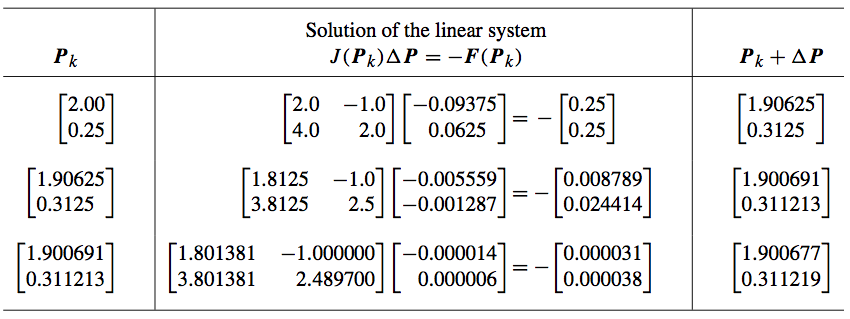
\includegraphics[width=100mm]{chap-2/tab_3-7.png}
\end{center}
\end{figure}
\begin{itemize}
\item Implementation of Newton's method can require the determination of several partial derivatives. 
\vspace{2mm}
\item It is permissible to use numerical approximations for the values of these partial derivatives, but care must be taken to determine the proper step size. 
\vspace{2mm}
\item In higher dimensions it is necessary to use the methods for solving linear systems introduced earlier in this chapter to solve for $\Delta P$. 
\end{itemize}
}

\frame{
\begin{itemize}
\item Programs 2.6 (Nonlinear Seidel Iteration) and 2.7 (Newton-Raphson Method) will require saving the nonlinear system $X = G(X)$, and the nonlinear system $F(X) = 0$ and its Jacobian matrix, $JF$, respectively, as M-files.
\item  As an example, consider saving the nonlinear system in Example 2.15 and the related Jacobian matrix as the M-files F.m and JF.m, respectively. 
\end{itemize}
}



%\frame{
%}


